\chapter{Implementation}

In this chapter we give a brief overview of the implementation of the algorithms presented above. In the prototyping phase, the asset allocation learning task has been implemented in Python as an extension of the PyBrain library. In a second phase, the architecture has been translated into C++ to achieve better performances. Here we only give an overview of the program, addressing the reader to the Git repository \url{www.github.com/pnecchi/Thesis} for the scripts and the detailed documentation. 

\section{Python Prototype}
\label{sec:python_prototype}

The first step of this project has been to implement a prototype in Python, a high-level, general-purpose, interpreted, dynamic programming language which is gaining a widespread popularity both in the academic world and in the industry. Python natively supports the object-oriented paradigm which makes it perfect to quickly develop a prototype of the class architecture, which can then be translated in C++. Moreover, thanks to external libraries such as Numpy, Scipy and Pandas, Python offers an open-source alternative to Matlab for scientific computing applications.\\
For the basic RL algorithms we exploited PyBrain\footnote{\url{http://pybrain.org/}}, a modular ML library for Python whose goal is to offer flexible, easy-to-use yet still powerful algorithms for ML tasks and a variety of predefined environments to test and compare different algorithms \cite{pybrain2010jmlr}. An RL task in PyBrain always consists of an \lstinline{Environment}, an \lstinline{Agent}, a \lstinline{Task} and an \lstinline{Experiment} interacting with each other as illustrated in Figure \ref{fig:pybrain}.\\
The \lstinline{Environment} is the world in which the \lstinline{Agent} acts and is characterized by a state which can be accessed through the \lstinline{getSensors()} method. The \lstinline{Agent} receives an observation of this state through the \lstinline{integrateObservation()} method and selects an action through the \lstinline{getAction()} method. This action is applied to the \lstinline{Environment} with the \lstinline{performAction()} method. However, the interactions between the \lstinline{Environment} and the \lstinline{Agent} are not direct but are mediated by the \lstinline{Task}. The \lstinline{Task} specifies what the goal is in an \lstinline{Environment} and how the agent is rewarded for its actions. Hence, the composition of an \lstinline{Environment} and a \lstinline{Task} fully defines the MDP. An \lstinline{Agent} always contains an \lstinline{Actor}, which represents the policy used to select actions. Based on the rewards that the \lstinline{Agent} receives via the \lstinline{getReward()} method, the \lstinline{Learner} improves the policy via a \lstinline{learn()} procedure. In this step, an \lstinline{Actor} may be used to evaluate a state with the goal of reducing the variance of the learning process. This entire learning process is controlled by an \lstinline{Experiment} object.\\ 
This structure is quite standard for a RL problem and can be easily adapted to the problem at hand and extended to the learning algorithms developed in this thesis. Based on this architecture, we thus developed a fully-working Python prototype of the asset allocation problem. This prototype yielded some interesting results both on simulated data and on historical data, in particular for the PGPE algorithm. However, the learning process resulted too slow to be run systematically for a large number of time-steps and training epochs. By consequent, we quickly decided to pass to C++.
\begin{figure}[t!]
	\centering
	\begin{tikzpicture}[node distance = 6em, auto, thick]
		\node (rect) at (0,0) [draw,thick,minimum width=8cm,minimum height=6cm] (Experiment) {};
		\node (rect) at (0,1.4) [draw,thick,minimum width=6cm,minimum height=2cm] (Task) {};
		\node (rect) at (0,1.4) [draw,thick,minimum width=3cm,minimum height=1cm] (Environment) {\lstinline{Environment}};
		\node (rect) at (0,-1.4) [draw,thick,minimum width=6cm,minimum height=2cm] (Agent) {};
		\node (rect) at (-1.9,-1.4) [draw,thick,minimum width=1.6cm,minimum height=1cm] (Critic) {\lstinline{Critic}};
		\node (rect) at (1.9,-1.4) [draw,thick,minimum width=1.6cm,minimum height=1cm] (Learner) {\lstinline{Learner}};
		\node (rect) at (0,-1.4) [draw,thick,minimum width=1.6cm,minimum height=1cm] (Actor) {\lstinline{Actor}};
		
		\draw (-2.8,3.3) node {\lstinline{Experiment}};
		\draw (-2.4,2.7) node {\lstinline{Task}};
		\draw (0.8,0) node {\lstinline{Action}};
		\draw (-2.25,1.7) node {\lstinline{State}};	
		\draw (2.7,0) node {\lstinline{Reward}};
		\draw (-2.4,-2.7) node {\lstinline{Agent}};
	
		\path [line] (Task.180) --++ (-0.5cm,0cm) |- node [near start]{\lstinline{Observation}} (Agent.180);
		\path [line] (Task.0) --++ (+0.5cm,0cm) |- (Agent.0);
		\draw[line] (Environment.180) -- (Task.180);
		\draw[line] (Agent.90) -- (Task.270); 
	\end{tikzpicture}
	\caption{PyBrain standard architecture for an RL problem.}
	\label{fig:pybrain}
\end{figure}

\section{C++ Implementation}
\label{sec:c++_implementation}
Passing from Python to C++ presents some challenges in the design of a suitable architecture for the RL algorithms discussed above. Following the approach of \cite{joshi2008c++}, our main goal has been code reusability, which is based on the important attributes of clarity and elegance of design. In addition, we always kept in mind the possibility that our original design might need to be extended in the future. In some cases we therefore favored extendability compared to efficiency. First we describe the C++ adaptation of the PyBrain's \lstinline{Environment}, \lstinline{Task}, \lstinline{Agent} and \lstinline{Experiment} objects with a particular attention to their concrete implementations for the asset allocation problem. Secondly, we discuss the design for an Average-Reward Actor-Critic agent (ARAC), which provides a concrete implementation of the \lstinline{Agent} interface.

\subsection{\lstinline{Environment}, \lstinline{Task}, \lstinline{Agent} and \lstinline{Experiment}}
Figure \ref{fig:class_architecture_base} schematically represents the design of the base components of an RL application, which closely replicates Pybrain's architecture. The pure abstract classes \lstinline{Environment}, \lstinline{Task}, \lstinline{Agent} and \lstinline{Experiment} define the generic interfaces to which all the concrete implementations of these objects must adhere. To achieve code modularity, we make most of the objects in our design clonable in order to allow for the polymorphic composition of classes. Exploiting this design pattern, we couple a \lstinline{Task} with an \lstinline{Environment} by storing a \lstinline{std::unique_ptr<Environment>} as a private member of the class. Similarly, an \lstinline{Experiment} is coupled via composition with a \lstinline{Task} and an \lstinline{Agent}. The methods of these classes are similar to those in Pybrain. For all the linear algebra operations we decided to use Armadillo\footnote{\url{http://arma.sourceforge.net/}}, a high quality linear algebra library which provides high-level syntax (API) deliberately similar to Numpy and Matlab aiming towards a good balance between speed and ease of use. Therefore, the state of the system and the actions performed by the agent are represented as \lstinline{arma::vector} objects. Let us now present the concrete implementation of these objects for the asset allocation task. \lstinline{MarketEnvironment} implements a financial market by storing the historical daily returns of the risky assets in an \lstinline{arma::matrix}. These values are read from a given input \lstinline{.csv} file, which is generated automatically running a Python script and which either contains real historical returns downloaded from Yahoo Finance\footnote{\url{https://uk.finance.yahoo.com/}} or synthetic returns generated according to a certain stochastic process. Therefore, we always work on samples of the system without making any assumption on its Markov transition kernel.
\begin{sidewaysfigure}[h!]
    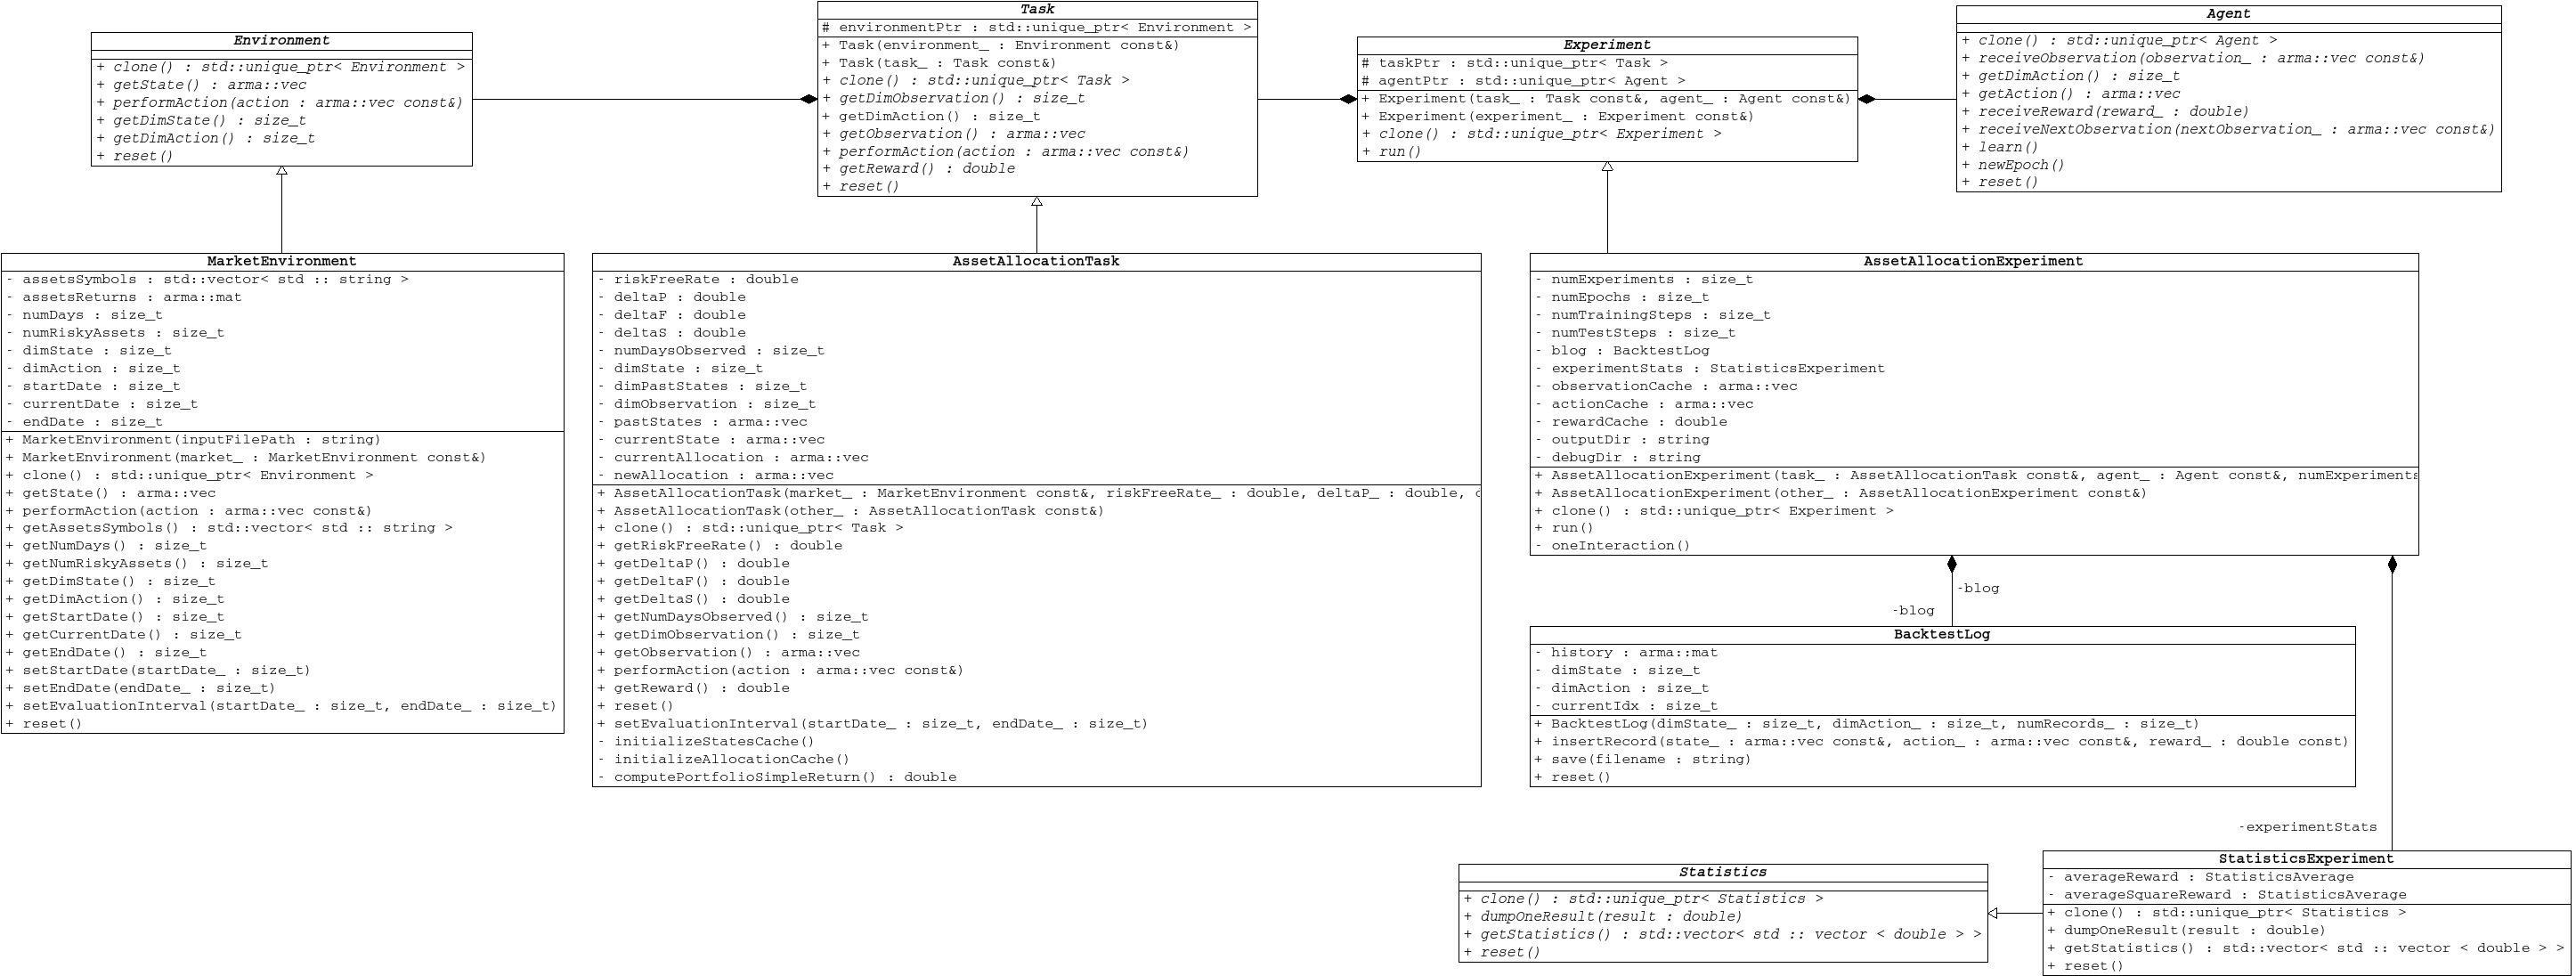
\includegraphics[width=\textwidth]{Images/A_agent_environment_interaction}
    \caption[Class architecture for the asset allocation problem.]{Class architecture for the learning process in the asset allocation problem.}
    \label{fig:class_architecture_base}
\end{sidewaysfigure}
\clearpage
The \lstinline{AssetAllocationTask} implements the MDP associated to the asset allocation problem by providing a method to compute the reward that the \lstinline{Agent} obtains from investing on the risky assets. The \lstinline{AssetAllocationTask} enlarges the system state so that the \lstinline{Agent} also observes the past $P$ states and the current portfolio weights. 
The \lstinline{AssetAllocationExperiment} handles the interactions between the \lstinline{Agent} and the \lstinline{AssetAllocationTask}. The learning process is divided in two phases: the training phase consists of a certain number of learning epochs over the same time period during which the \lstinline{Agent} improves the parameters of its policy via the \lstinline{learn} method. Some estimates of the objective function are dumped in the \lstinline{StatisticsExperiment} object and are used in the post-processing phase to plot the learning curves of the algorithm. In the backtest phase, the \lstinline{Agent} applies the learned policy on the time period which follows the one used for training and the relevant performance measures are stored in the \lstinline{BacktestLog} for successive analysis and comparison between different learning algorithms.

\subsection{\lstinline{ARACAgent}}
A concrete implementation of the \lstinline{Agent} interface completes the standard structure of an RL task. In this section we discuss the design for an Average Reward Actor-Critic agent (ARAC), which includes most of the features of the other algorithms tested in this thesis. The full architecture of this agent is illustrated in Figure \ref{fig:class_architecture_arac}, but for brevity we will only focus on the more interesting aspects.\\
The \lstinline{ARACAgent} builds upon a \lstinline{StochasticActor} and a \lstinline{Critic} via composition. A \lstinline{StochasticActor} is simply a wrapper around a \lstinline{StochasticPolicy}, a pure abstract class defining the generic interface for a stochastic policy used by an agent to select actions. In addition to \lstinline{getAction} and get/set methods for the policy parameters, a \lstinline{StochasticPolicy} must implement the \lstinline{likelihoodScore} method which computes the likelihood score $\nabla_\theta \log \pi_\theta(s,a)$ for a given state and action and which plays a crucial role in any policy gradient algorithm.\\
We provide two examples of concrete implementations of the \lstinline{StochasticPolicy}. The first example is the \lstinline{BoltzmannPolicy} typically used in discrete action spaces. The implementation of this policy is quite straightforward and we won't discuss the details. The second and more interesting stochastic policy implemented is the \lstinline{PGPEPolicy}. This class is based on the decorator design pattern which is typically used to extend the interface of a certain class. Indeed, the \lstinline{PGPEPolicy} is a \lstinline{StochasticPolicy} which contains by polymorphic composition a \lstinline{Policy}, a pure abstract class which provides the generic interface for a policy, potentially deterministic. This \lstinline{Policy} object represents the deterministic controller $F_\theta$ used in the PGPE algorithm. Moreover, the \lstinline{PGPEPolicy} contains by polymorphic composition a \lstinline{ProbabilityDistribution}, a pure abstract class defining the generic interface for a probability distribution. This probability distribution represents the hyper-distribution $p_\xi$ on the controller parameters. In order to be used in a PGPE algorithm, a \lstinline{ProbabilityDistribution} must implement a \lstinline{likelihoodScore} method to compute the likelihood score of the hyper-distribution $\nabla_\xi \log p_\xi(\theta)$. Hence, the \lstinline{likelihoodScore} method of \lstinline{PGPEPolicy} simply broadcasts the call to the \lstinline{likelihoodScore} method of its underlying \lstinline{ProbabilityDistribution}. A concrete implementation of a \lstinline{ProbabilityDistribution} is provided by the \lstinline{GaussianDistribution}, which implements a multi-variate and axis-aligned normal distribution $\calN(\mu, \diag(\sigma))$.\\
The objects discussed so far are sufficient to implement an actor-only learning algorithm, potentially using a baseline to evaluate the rewards. A more advanced variance reduction technique consists in using a \lstinline{Critic}, which approximates the value function and provides an evaluation of a given state. The \lstinline{Critic} class is simply a wrapper around a \lstinline{FunctionApproximator} which provides a generic interface for a parametric function $B_\omega(s)$. The key methods of this class are \lstinline{evaluate}, which evaluates the approximator at a given point, and \lstinline{gradient}, which computes its gradient at a given point.\\
Finally, the \lstinline{ARACAgent} employs some \lstinline{LearningRate} to control the speed of the gradient descent optimization algorithm. A naive approach is to use a \lstinline{ConstantLearningRate}, but this leads to a large-variance in the objective function value attained by the stochastic optimization algorithm. A more sensible choice is to use a \lstinline{DecayingLearningRate} which decreases with the number of learning epochs performed by the agent according to $\alpha_n = \frac{a}{n^b}$. In this way, the learning process progressively ``cools down'' (using a simulated annealing terminology) and stabilizes to a given policy. This concludes our quick overview of the class architecture used for this project. In the thesis, other applications and algorithms were considered and we refer the reader to the full document for a more complete discussion.
\begin{sidewaysfigure}[ht]
    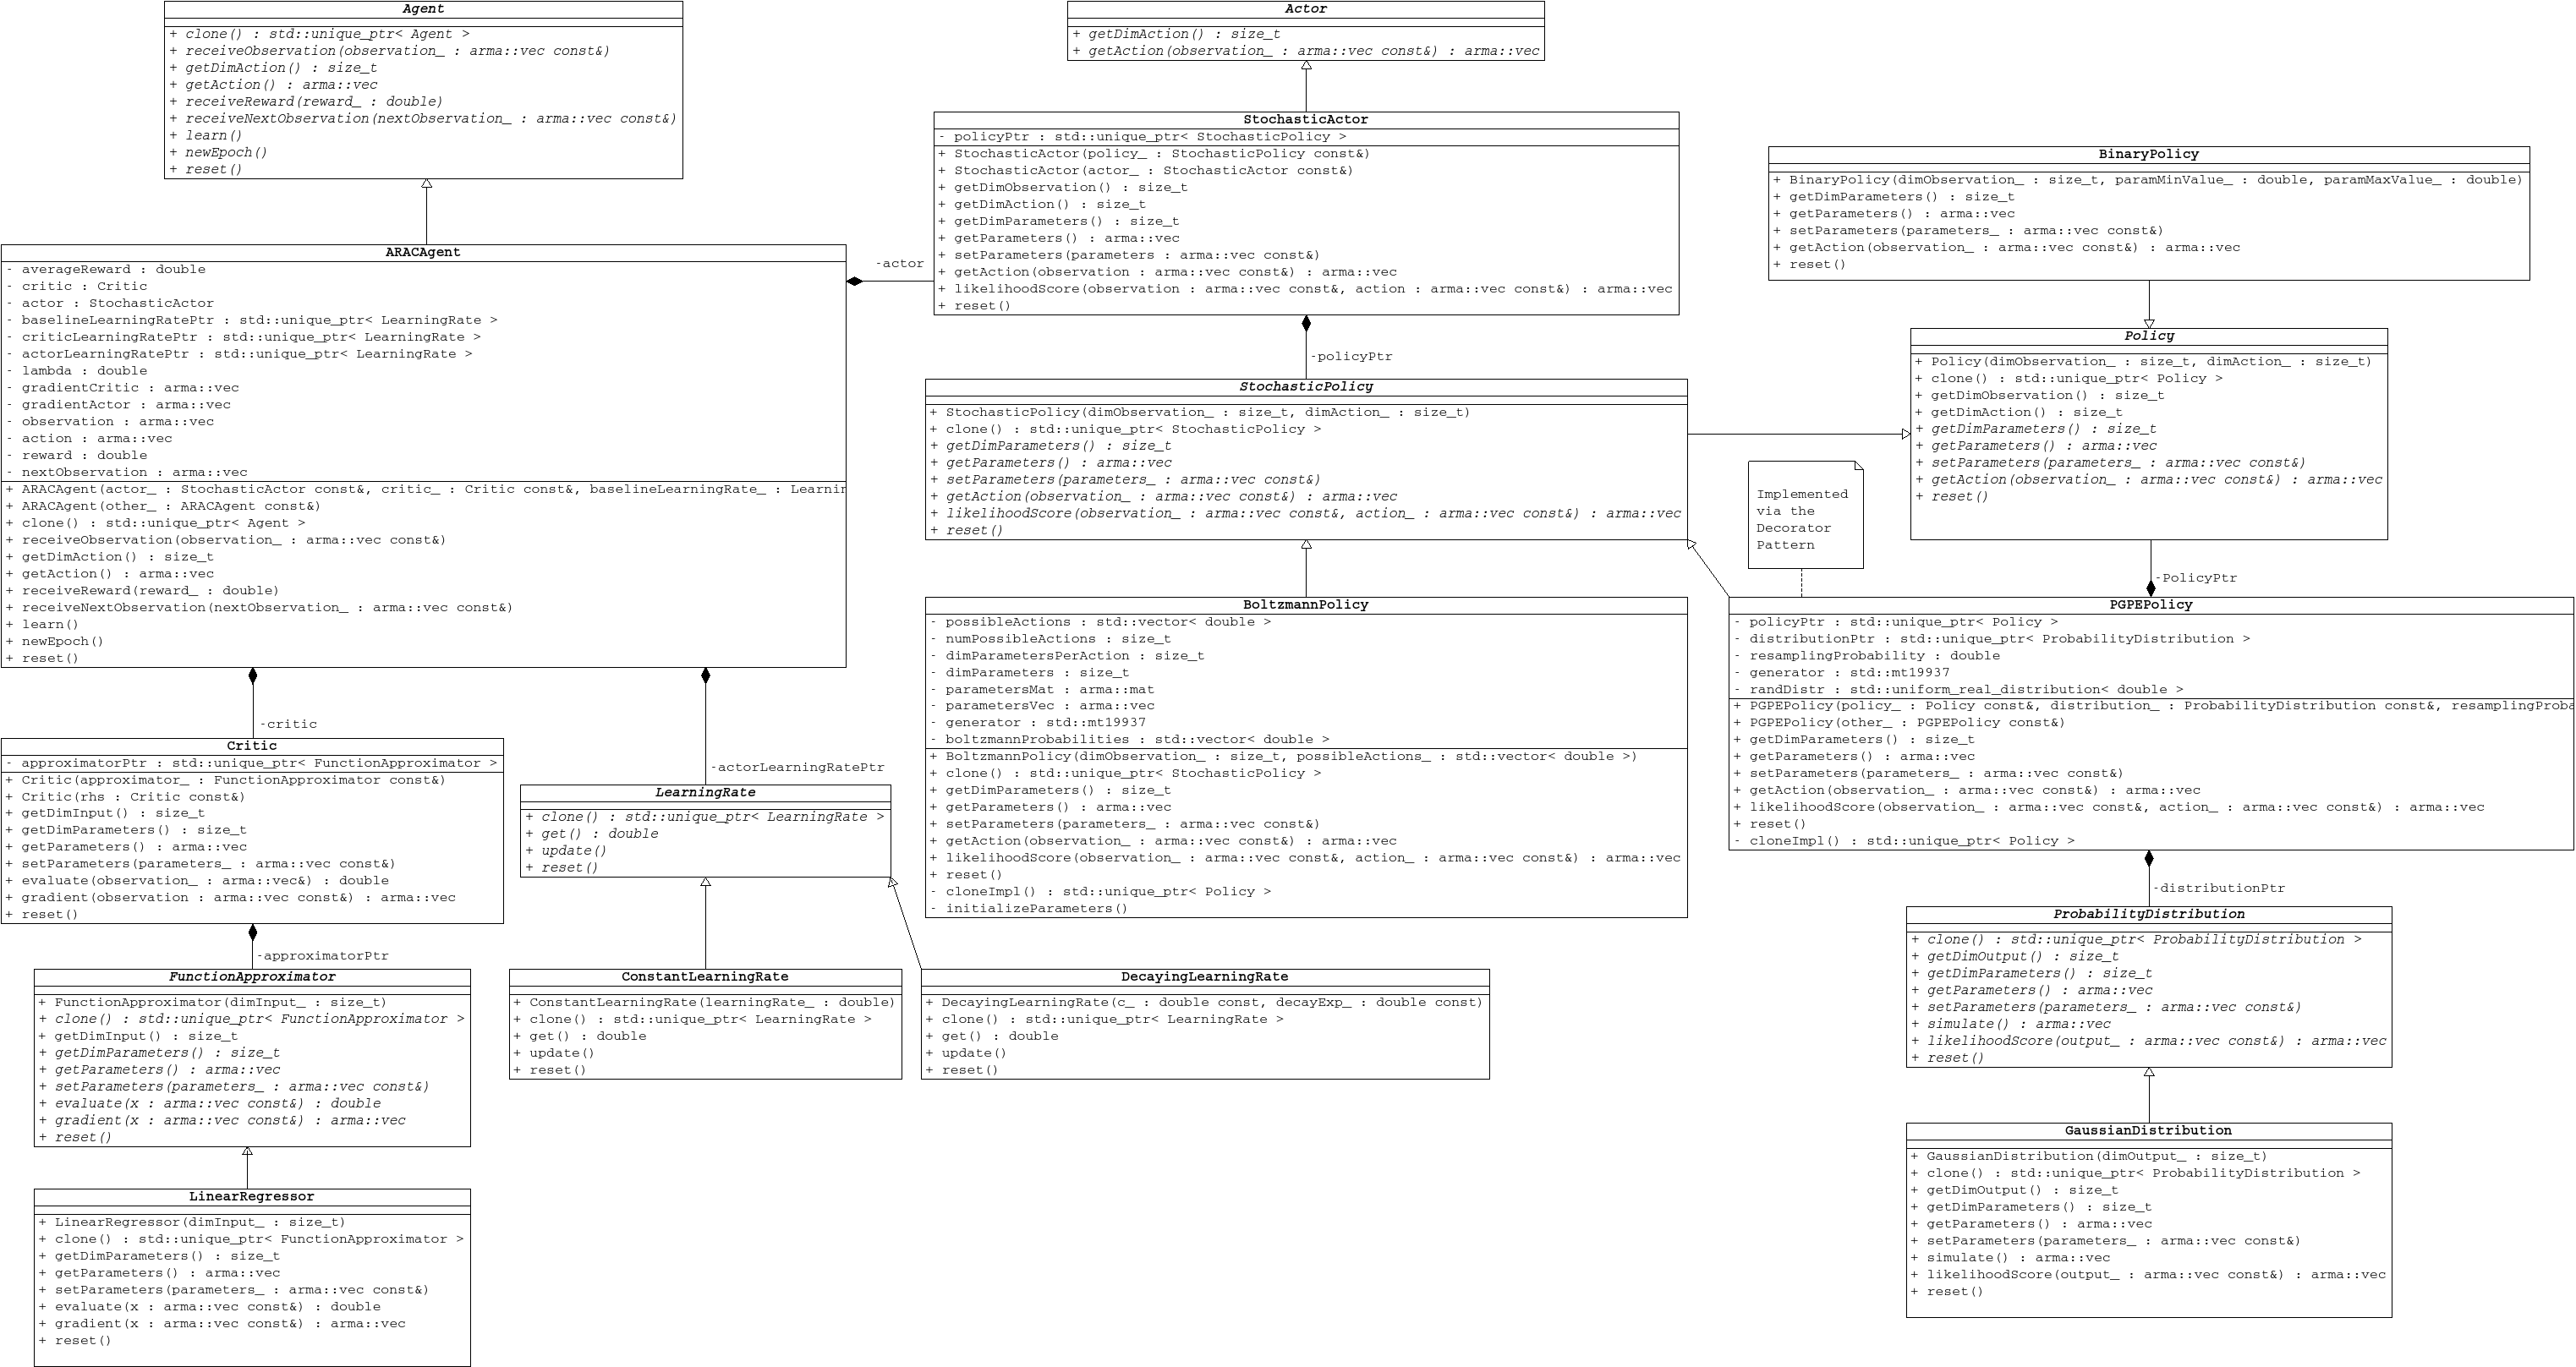
\includegraphics[width=\textwidth]{Images/A_agent}
    \caption[Class architecture for an ARAC agent]{Class architecture for an Average Reward Actor-Critic agent (ARAC).}
    \label{fig:class_architecture_arac}
\end{sidewaysfigure}
\clearpage

\section{Execution Pipeline}
\label{sec:execution_pipeline}

In this section we describe the full pipeline of the program, which is schematically represented in Figure \ref{sec:execution_pipeline}. This pipeline allows to run the learning algorithm for the asset allocation problem and automatically determine a trading strategy. The execution consists of the following steps. 

\subsection{Compilation} To build the \lstinline{thesis} library it is sufficient to run the \lstinline{Makefile} generated with \lstinline{cmake}. This produces two executables: \lstinline{main} which is used to debug the program in the \lstinline{Code::Blocks} IDE and \lstinline{main_thesis} which is used to run the experiment in the full execution pipeline. 

\subsection{\lstinline{generate_synthetic_series.py}} This Python script simulates the returns of a synthetic asset and prints them on a \lstinline{.csv} file which is then read by \lstinline{main_thesis} and used to initialize the \lstinline{MarketEnvironment} object. Alternatively, \lstinline{market_data_collector.py} collects the historical returns for a list of given assets from Yahoo finance.

\subsection{\lstinline{experiment_launcher.py}} This Python script manages the execution pipeline. First, the experiment parameters are specified and dumped in a \lstinline{.pot} file which is then read by \lstinline{main_thesis}. Given the parameter values, the script determines the folders where the output should be written so that the results can be easily associated to a specific set of parameters. Subsequently, it launches the \lstinline{main_thesis} executable passing the correct parameters via the command line. Finally it runs the \lstinline{postprocessing.py} scripts which processes the output files.  

\subsection{\lstinline{main_thesis}} This executable takes some inputs from the command line, such as the algorithm to use, the paths to the input files and the paths where the output files should be generated. The experiment parameters are then read from the \lstinline{.pot} file generated by the \lstinline{experiment_launcher.py} using \lstinline{GetPot}. The type of learning algorithm is specified by a string passed to the executable via command line and then used by the factory \lstinline{FactoryOfAgents} to instantiate the corresponding \lstinline{Agent}. When the \lstinline{AssetAllocationExperiment} is run, it outputs various statistics to the given destination folders. More in detail, it prints two files for every independent run of the experiment: a \lstinline{debug.csv} file which contains the learning curves of the algorithm and an \lstinline{output.csv} file which contains the backtest performance measures for the trading strategy learned by the \lstinline{Agent} during training.   

\subsection{\lstinline{postprocessing.py}} This Python script processes the various files produced by \lstinline{main_thesis} and generates an aggregate analysis of the various learning algorithms, so that they can be easily compared and assessed. In particular, it computes the average and confidence intervals for the learning curves of the algorithms and the backtest cumulative profits of the learned strategies. Moreover, it computes some performance measures typically used in Finance to evaluate a trading strategy, such as the Sharpe ratio and the maximum drawdown. The results of this analysis are stored in some \lstinline{.csv} files and some images are generated using the Python library \lstinline{matplotlib}. 


\begin{sidewaysfigure}[t!]
	\centering
	\resizebox{\textwidth}{!}{%{ %
	\begin{tikzpicture}[node distance = 6em, auto, thick]
		\node (rect) at (-9.5,-2) [draw,very thick,minimum width=3cm,minimum height=3cm] (generate_synthetic_series) {};
		\node (rect) at (0,0) [draw,very thick,minimum width=15cm,minimum height=10cm] (experiment_launcher) {};
		\node (rect) at (+9,-2) [GloriousGreen,draw,very thick,minimum width=2cm,minimum height=3cm] (convergence) {};
		\node (rect) at (+9,+2) [GloriousGreen,draw,very thick,minimum width=2cm,minimum height=3cm] (performance) {};
		\node (rect) at (-6,2) [GloriousGreen,draw,very thick,minimum width=2cm,minimum height=3cm] (input) {};
		\node (rect) at (-6,-2) [GloriousGreen,draw,very thick,minimum width=2cm,minimum height=3cm] (synthetic) {};
		\node (rect) at (-2,0) [SteelBlue, draw,very thick,minimum width=4cm,minimum height=8cm] (main_thesis) {};
		\node (rect) at (2,2) [GloriousGreen,draw,very thick,minimum width=2cm,minimum height=3cm] (output) {};
		\node (rect) at (2,-2) [GloriousGreen,draw,very thick,minimum width=2cm,minimum height=3cm] (debug) {};
		\node (rect) at (5.5,0) [draw,very thick,minimum width=3cm,minimum height=3cm] (postprocessing) {};
		
		\draw (0,5.5) node {\lstinline{experiment_launcher.py}};
		\draw (-9.5,0) node {\lstinline{generate_synthetic_series.py}};
		\draw (-6,-4) node {\lstinline{synthetic.csv}};
		\draw (-7.8,4) node {\lstinline{Single_Synth_RN_P0_F0_S0_N5.pot}};	
		\draw (5.5,2) node {\lstinline{postprocessing.py}};
		\draw (2,4) node {\lstinline{output.csv}};
		\draw (2,-4) node {\lstinline{debug.csv}};
		\draw (9.5,4) node {\lstinline{performance.csv}};
		\draw (9.5,-4) node {\lstinline{convergence.csv}};
		\draw (-2,0) node {\lstinline{main_thesis}};	
	
		\draw[line] (generate_synthetic_series.0) -- (synthetic.180);
		\draw[line] (debug.0) -- (postprocessing.180);
		\draw[line] (output.0) -- (postprocessing.180);
		\draw[line] (postprocessing.0) -- (performance.180);
		\draw[line] (postprocessing.0) -- (convergence.180);
		\draw[line] (input.0) -- (main_thesis.135);
		\draw[line] (synthetic.0) -- (main_thesis.225);
		\draw[line] (main_thesis.45) -- (output.180);
		\draw[line] (main_thesis.315) -- (debug.180);
	\end{tikzpicture}
	}
	\caption[Execution pipeline of an asset allocation experiment]{Execution flow of an asset allocation experiment. Black boxes denote  Python scripts, blue boxes executables while red boxes input/output files.}
	\label{fig:pybrain}
\end{sidewaysfigure}